\section{Reach-avoid flight}

\subsection*{(a)}
Only the \(v_y\) and \(\omega\) dynamics depend on the thrusts. In the Hamiltonian,
the terms involving \(T_1,T_2\) are linear:
\[
\left(\frac{p_{v_y}\cos\phi}{m}-\frac{p_\omega \ell}{I_{yy}}\right)T_1
+
\left(\frac{p_{v_y}\cos\phi}{m}+\frac{p_\omega \ell}{I_{yy}}\right)T_2
\]
So each thrust is chosen at one of its bounds. If the coefficient is negative,
use max thrust; otherwise use min thrust.% This gives the bang-bang controller
%implemented in \texttt{optimal\_control}.

\subsection*{(b)}
For the target set
\[
T=[3,7]\times[-1,1]\times[-\pi/12,\pi/12]\times[-1,1]
\]
I used
\[
h(x)=\max\{3-y,\ y-7,\ |v_y|-1,\ |\phi|-\pi/12,\ |\omega|-1\}
\]
Then \(h(x)\le 0\) exactly when all target constraints are satisfied.

\subsection*{(c)}
For the envelope
\[
E=[1,9]\times[-6,6]\times[-\infty,\infty]\times[-8,8]
\]
I used
\[
e(x)=\max\{1-y,\ y-9,\ |v_y|-6,\ |\omega|-8\}
\]
There is no pitch constraint in the envelope, so \(\phi\) does not appear.

\subsection*{(d)}
The zero isosurface separates states that can reach the target while staying in
the envelope from states that cannot. The tilted ridge/valley comes from the
coupling between pitch, angular rate, and vertical acceleration. For example,
when the quadrotor is tilted, thrust is not purely vertical, so the same vertical
velocity can be recoverable or unrecoverable depending on whether \(\phi\) and
\(\omega\) are rotating the vehicle back toward level flight or farther away
from it.

\begin{figure}[H]
\centering
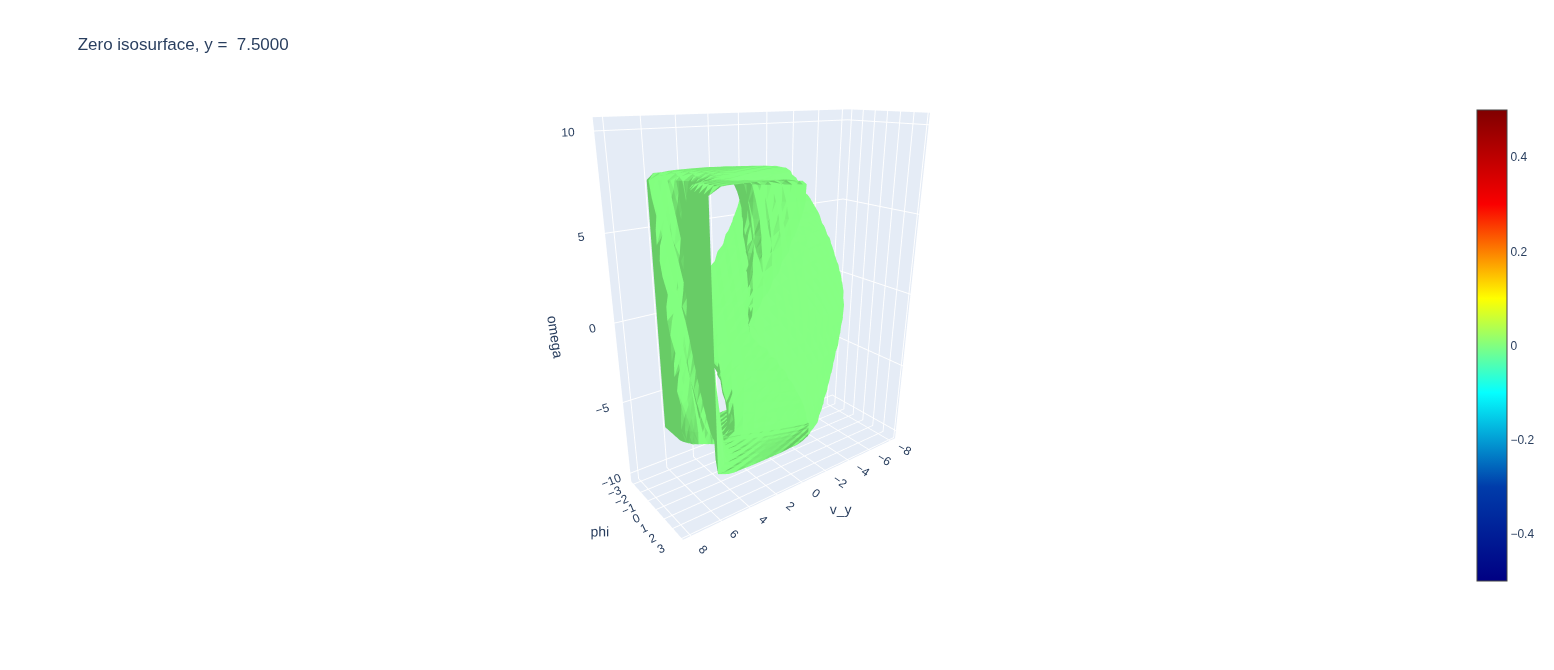
\includegraphics[width=0.65\textwidth]{figures/isosurface.png}
\caption{Zero isosurface of the reach-avoid value function}
\label{fig:hj_isosurface}
\end{figure}

\subsection*{(e)}
Dynamic programming gives a global feedback policy over the grid, so online
control is cheap once the value function is computed. The downside is that the
offline solve is expensive in time and memory, especially as the state dimension
increases. MPC is usually easier to adapt online to new constraints or obstacles,
but it solves an optimization problem at each time step and is more local.

\subsection*{Code}
Code in \hyperref[hj_reachability]{Appendix}.
